\chapter{Preeliminary Results}

\subsection{Hasil Prediksi Menggunakan Neural Network}

\begin{center}
\begin{tabular}{|l|l|}
\hline
Hasil Pengukuran & Prediksi \\ \hline
5.5 & 4.100310325622559 \\ \hline
8.4 & 6.7429656982421875 \\ \hline
3.2 & 2.2476131916046143 \\ \hline
7.2 & 5.995209693908691 \\ \hline
2.5 & 2.245391607284546 \\ \hline
4.0 & 3.344273090362549 \\ \hline
5.6 & 5.625854015350342 \\ \hline
9.0 & 6.900030136108398 \\ \hline
2.0 & 3.1297378540039062 \\ \hline
4.1 & 6.302687168121338 \\ \hline
5.5 & 6.865676403045654 \\ \hline
4.3 & 2.2473692893981934 \\ \hline
4.6 & 4.0304718017578125 \\ \hline
7.5 & 5.180098533630371 \\ \hline
8.3 & 6.900175094604492 \\ \hline
\end{tabular}
\end{center}

\subsection{Perbandingan dengan metode BOUSS-2D}
\begin{center}
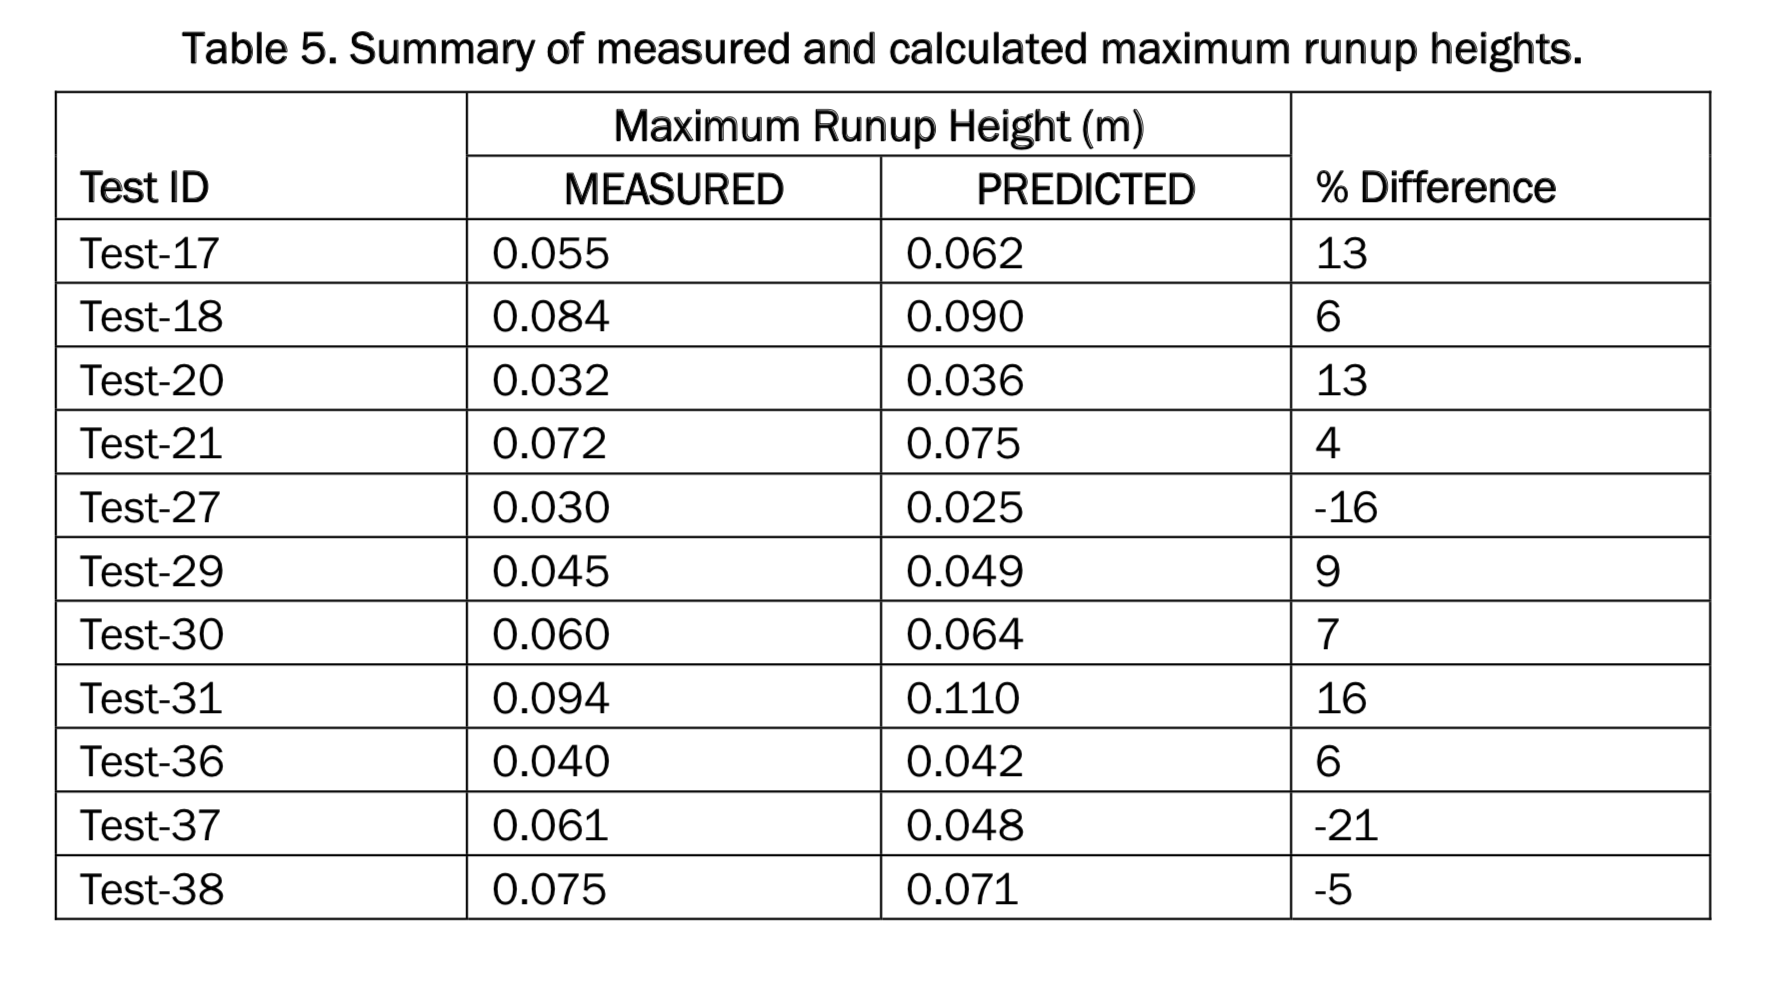
\includegraphics{table}
\end{center}